\documentclass[]{article}


\usepackage[italian]{babel}% package per la lingua italiana
\usepackage{graphicx} % package per caricare immagini 
\usepackage{tabularx} % package per creare tabelle 
\usepackage[utf8x]{inputenc} % package per i simboli utf8x
\usepackage{times} % package per il times new roman font
\usepackage{float} %serve per mettere le immagini in posizione Here
\usepackage{color} % per colorare il testo
\usepackage{pgf, tikz}
\usetikzlibrary{arrows, automata}
\usepackage{eurosym}
\usetikzlibrary{arrows.meta}
\usepackage{amsmath}

\begin{document}

\title{Set 2 Algoritmi}
\author{Cracco Andrea VR432685\\Alberto Purrone VR433409\\Litterini Simone VR439416\\}
\date{\today}
\maketitle




\section{Exercise 1}

Provide a linear time algorithm that takes in input a weighted directed graph $G = (V, E)$, with costs on theedges $c(e)$ for $e∈E$ (cost may be negative), a node $t∈V$ and, for each $v∈V$ a value $d(v)$,and decides whether for each $v ∈ V$ it is true that $d(v)$ is the cost of the path of minimum cost among all the paths from from v to t.

\subsection{First Observation}

We change the cost of each edge $e(v,w)$ according to the formula $$ c_{new}(e) = c(e)-d(v)+d(w)$$ 

\begin{itemize}

\item if $c_{new}(e)  < 0$ the minimum cost didn't take in account the edge because $d(w) - d(v)$ is greather than the cost of the current edge so the cost are not correct;

\item if $c_{new}(e)  = 0$ the minimum path from v to t passes through this edge;

\item if $c_{new}(e)  > 0$ the edge is not part of the minimum path from v to t;


\end{itemize}

\subsection{Second Observation}

If there exist a path from v to t of cost c and we reverse all the edges, there should be a path from t to v with cost c;

\subsection{Algorithm}

\begin{enumerate}

\item Suppose that if t is not reachable from a vertex v, $ d(v) = + \infty$;
\item For each edge $e(v,w)$, change its cost to $ c_{new}(e) $;

\item Reverse the direction of all edges;

\item Starting from t, do a modified DFS in the following way:

\item For each edge $e(v,w)$ that is outgoing from the current vertex v:

\begin{itemize}


\item If $c_{new}(e) = 0$: visit the node w
\item If $c_{new}(e) < 0$: return false
\item If $c_{new}(e) > 0$: ignore the edge

\end{itemize}
 
\item If there exist a node v not visited by the algorithm such that $d(v) < +\infty$: return false;
\item Return true;


\end{enumerate}


\section{Exercise 2}

You are given a weighted directed graph $G = (V, E)$, with costs on the edges $c(e) for e ∈ E$ (cost may
be negative), a node $t ∈ V$ and, for each $v ∈ V$ a value d(v) which is the cost of a path of minimum cost
from v to t. Provide an $O(|E| log |V |)$ algorithm that given G, $d()$ and a node t 6 = t 0 computes, for each
$v ∈ V$ the minimum cost of a path from v to t 0. 

\subsection{}





\section{Exercise 3}

Show that if we apply the algorithm seen in class to find the min-cost circulation for the network shown
in the figure, there exist a sequence of choices of the cycle along which we improve that require $2*10^6$
iteration to solve the problem.



\begin{figure}[H]
	\begin{center}
		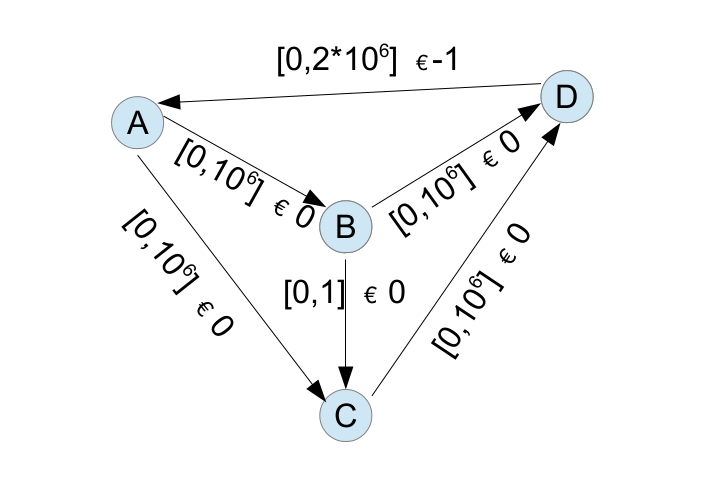
\includegraphics[width=0.6\textwidth]{abcd.png}
		\caption{Flow network(N) of the problem }
		
	\end{center}
\end{figure}


\subsection{Algorithm}

The steps of the algorithm saw in the class are:
\begin{enumerate}

\item Find a Feasible circulation $Fc$ for N 
\item While $R(Fc)$ has no negative cycle C, then $Fc = Sw(Fc,C)$

\end{enumerate}



The fist step of the algorithm saw in the class is to produce the residual graph 


\begin{tikzpicture}[
  ->,
  >=stealth',
  shorten >=1pt,
  auto,
  node distance=2.8cm,
  semithick,
  every state/.style={fill=red,draw=none,text=white},
]

        \tikzstyle{every state}=[
            draw = black,
            thick,
            fill = white,
            minimum size = 2mm
        ]

        \node[state] (a) {$A$};
        \node[state] (b) [right of=a]{$B$};
        \node[state] (c) [below right of=a]{$C$};
        \node[state] (d) [right of=b]{$D$};


        \path[every node/.style={sloped,anchor=south,auto=false}] (a) edge node {\tiny$[0,(10^6)-1]$    \euro{0}} (b);
        \path[every node/.style={sloped,anchor=south,auto=false}] (a) edge node {\tiny$[0,10^6] $    \euro{0}} (c);
        \path[every node/.style={sloped,anchor=south,auto=false}] (b) edge node {\tiny$[0,10^6] $    \euro{0}} (d);
        \path[every node/.style={sloped,anchor=south,auto=false}] (c) edge node {\tiny$[0,(10^6)-1] $    \euro{0}} (d);
        \path[every node/.style={sloped,anchor=south,auto=false}] (c) edge node {\tiny$[0,1]$    \euro{0}} (b);
        \path[every node/.style={sloped,anchor=south,auto=false}] (d) edge [bend right = 35] node {\tiny$[0,(2*10^6)-1]$    \euro{-1}} (a);

	\path[every node/.style={sloped,anchor=south,auto=false}] (b) edge [bend right] node {\tiny$1$    \euro{0}} (a);
	\path[every node/.style={sloped,anchor=south,auto=false}] (d) edge [bend left=25] node {\tiny$1 $    \euro{0}} (c);
	\path[every node/.style={sloped,anchor=south,auto=false}] (a) edge [bend right] node {\tiny$1$    \euro{0}} (c);
	\path[every node/.style={sloped,anchor=south,auto=false}] (a) edge [bend left=60] node {\tiny$1$    \euro{0}} (d);

 \end{tikzpicture}

the graph above is the result of the first iteration of the worst choice that the algoithm can do.

\begin{tikzpicture}[
  ->,
  >=stealth',
  shorten >=1pt,
  auto,
  node distance=2.8cm,
  semithick,
  every state/.style={fill=red,draw=none,text=white},
]

        \tikzstyle{every state}=[
            draw = black,
            thick,
            fill = white,
            minimum size = 2mm
        ]

        \node[state] (a) {$A$};
        \node[state] (b) [right of=a]{$B$};
        \node[state] (c) [below right of=a]{$C$};
        \node[state] (d) [right of=b]{$D$};


        \path[every node/.style={sloped,anchor=south,auto=false}] (a) edge node {\tiny$[0,(10^6)-1]$    \euro{0}} (b);
        \path[every node/.style={sloped,anchor=south,auto=false}] (a) edge node {\tiny$[0,(10^6)-1]$    \euro{0}} (c);
        \path[every node/.style={sloped,anchor=south,auto=false}] (b) edge node {\tiny$[0,(10^6)-1]$    \euro{0}} (d);
        \path[every node/.style={sloped,anchor=south,auto=false}] (c) edge node {\tiny$[0,(10^6)-1] $    \euro{0}} (d);
        \path[every node/.style={sloped,anchor=south,auto=false}] (b) edge node {\tiny$[0,1]$    \euro{0}} (c);
        \path[every node/.style={sloped,anchor=south,auto=false}] (d) edge [bend right = 35] node {\tiny$[0,(2*10^6)-2]$    \euro{-1}} (a);

	\path[every node/.style={sloped,anchor=south,auto=false}] (b) edge [bend right] node {\tiny$1$    \euro{0}} (a);
	\path[every node/.style={sloped,anchor=south,auto=false}] (d) edge [bend left=25] node {\tiny$1 $    \euro{0}} (c);
	\path[every node/.style={sloped,anchor=south,auto=false}] (a) edge [bend right] node {\tiny$1$    \euro{0}} (c);
	\path[every node/.style={sloped,anchor=south,auto=false}] (a) edge [bend left=60] node {\tiny$2$    \euro{0}} (d);
	\path[every node/.style={sloped,anchor=south,auto=false}] (d) edge [bend right] node {\tiny$1$    \euro{0}} (b);



 \end{tikzpicture}

the second graph is the second iteration and if we continue to take the path from A to D passing each time from the edge between B and C 
( the path ABCD and ACBD )
the result is a repeat of this two iterations above and using this choice we have that the algorithm takes $2*10^6$ iterations


\section{Exercise 4}

Assume that the following matrix has to be tested for the C1P. Using the algorithm seen in class provide 
\begin{enumerate}

\item[a] The overlap graph
\item[b] The containment graph

\end{enumerate}

If the matrix has the C1P, provide 3 distict permutations of the columns that leave the 1s consecutive
in each row (if there are fewer than 3 possible such permutations, provide them all). If the matrix does not have the C1P then apply the gap minimization algorithm considering only the last 5 columns.

%\[
%
%A=
%\left[ {\begin{array}{ccccccccc}
%
%1 & 1 & 1 & 0 & 1 & 1 & 0 & 1 & 1 \\
%1 & 1 & 1 & 1 & 1 & 1 & 0 & 0 & 1 \\
%0 & 1 & 1 & 0 & 1 & 0 & 0 & 0 & 0 \\
%0 & 1 & 0 & 0 & 0 & 1 & 0 & 0 & 1 \\
%1 & 1 & 1 & 0 & 1 & 1 & 1 & 1 & 0 \\
%0 & 1 & 0 & 0 & 0 & 0 & 0 & 0 & 0 \\
%0 & 0 & 0 & 0 & 1 & 0 & 0 & 0 & 0 \\
%
%\end{array} } \right]
%
%\]
%
%

%\begin{matrix}
%
%1 & 1 & 1 & 0 & 1 & 1 & 0 & 1 & 1 \\
%1 & 1 & 1 & 1 & 1 & 1 & 0 & 0 & 1 \\
%0 & 1 & 1 & 0 & 1 & 0 & 0 & 0 & 0 \\
%0 & 1 & 0 & 0 & 0 & 1 & 0 & 0 & 1 \\
%1 & 1 & 1 & 0 & 1 & 1 & 1 & 1 & 0 \\
%0 & 1 & 0 & 0 & 0 & 0 & 0 & 0 & 0 \\
%0 & 0 & 0 & 0 & 1 & 0 & 0 & 0 & 0 
%
%\end{matrix}

\subsection{overlap graph}

\begin{figure}[H]
	\begin{center}
		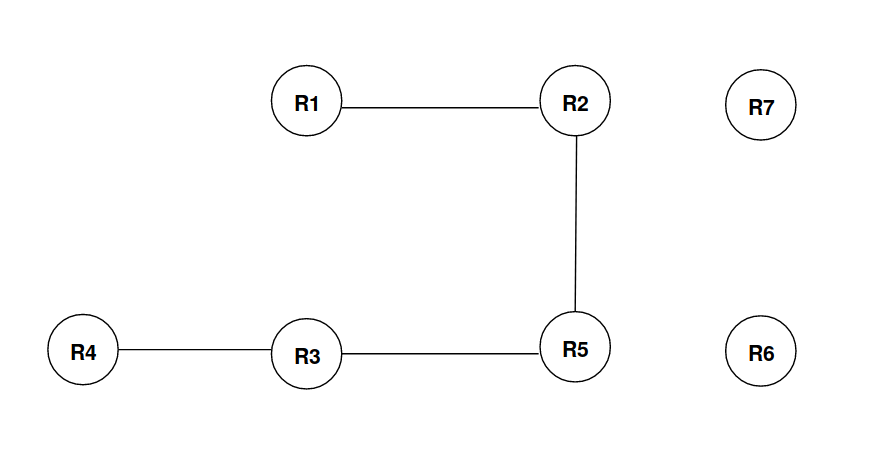
\includegraphics[width=0.6\textwidth]{overlap_graph.png}
	\end{center}
\end{figure}


\subsection{containment graph}







\section{Exercise 5}

%A lab is seriously facing shortage of primary storage space for its files/data. The lab has to buying/rent
%secondary remote storage facilities. Preliminary analyses have indicated this as a better solution than
%in-house expansion of the primary storage. The different available options have both limitations in the
%maximum amount of space offered and costs related to the access of the information, once stored there.
%We are interested in determining the optimal policy to choose how to distribute the files not anymore
%fitting in-house on different secondary remote storage facilities in order to limit the cost incurred by taking
%into account the different expected usage rate of the different type of information we are relocating.
%Assume there are n remote facilities where to relocate the exceeding files. Let α j be the maximum
%amount of information on the remote facility j and χ j be the cost to access one unit of information
%from this facility. We assume that the information we need to store remotely is divided into m different
%categories, each one of which is accessed with some rate. Let γ i be the amount of information units from
%the category i, and let ρ i be the rate (how many times per unit time) a unit of information from category
%i will need to be retrieved. We aim at storing/distributing the information in the different remote storage
%places in order to minimize the overall expected cost of retrieval.
%
%


















\end{document}

